% SSEE — Paper 4: Algebraic Derivation of CMB Background from φ and π — Peer-Review Corrected
% Compile: pdflatex SSEE_Paper4_ToE.tex (×2) + bibtex
\documentclass[12pt,a4paper]{article}

\usepackage{amsmath,amssymb,amsfonts,amsthm}
\newtheorem{conjecture}{Conjecture}
\usepackage{graphicx}
\graphicspath{{../results/figures/}}
\usepackage{booktabs}
\usepackage[colorlinks=true,linkcolor=red!70!black,citecolor=green!50!black,urlcolor=blue!80!black]{hyperref}
\usepackage{xcolor}
\usepackage{geometry}
\usepackage{natbib}
\usepackage{caption}
\usepackage{float}
\usepackage{array}
\usepackage{tcolorbox}
\usepackage{tabularx}
\usepackage{microtype}

\geometry{margin=2.5cm}

\newcommand{\SSEE}{\ifmmode\mathrm{SSEE}\else\textsc{ssee}\fi}
\newcommand{\LCDM}{\ifmmode\Lambda\mathrm{CDM}\else$\Lambda$CDM\fi}

% ---------------------------------------------------------------
\title{\textbf{Structural Self-Energy Expansion as a Two-Axiom Cosmology:\\
Algebraic Derivation of the CMB Background from~$\varphi$ and~$\pi$}\\[0.5em]
\normalsize SSEE — Paper~4 (Peer-Review Corrected)}

\author{Mike Edison Almeida Vallejo \\
\small \textit{Independent Researcher} \\
\small \href{mailto:mike.almeida1721@gmail.com}{mike.almeida1721@gmail.com} \\
\small ORCID: \href{https://orcid.org/0009-0008-2195-7836}{0009-0008-2195-7836}
}
\date{2026}
% ---------------------------------------------------------------

\sloppy
% abstract a todo el ancho (ahorra líneas → cabe en la página del título)
\renewenvironment{abstract}
  {\begin{center}\textbf{\abstractname}\end{center}\par\small\noindent\ignorespaces}
  {\par\medskip}
% ACTA-PROCEDENCIA {"commit": "5651fc97a90dc17d52be0317b46142db9ac86fcb", "reproducible_desde_commit": true, "cambios_sin_commitear": [], "script": "src/valores_tex.py", "script_sha256": "cb5ceb2369bdef5e586d471d57d44a11a9fed354be540a96ce34da85e582efa4", "nucleo_sha256": "5cec8af72d88f154116c5a532e42a9b6ff7a5b4c3d86bcc6921eabb246698993", "entradas": {"manuscript/valores.yaml": "5fa01e91dd68164243d664a73264bb6c87431d2ec0bd69db87c62a983a55992d", "results/logs/kids_publicados.json": "6c25c98059ce91038215358b4e7ac9cfb40198f410354937cee4ea00b46654ff", "results/logs/p10_uv_fscreen.json": "8fb68b295c848e0292e5701e7de795ba7c7ba25e3292d776260bb3dea8970c95", "results/logs/s8_desde_b1.json": "6d225f4403fbfbe6934d7edca26aaefbbe19e05ef6c7b7eda842a259e798b1c1"}, "argv": ["src/valores_tex.py"], "fecha": "2026-09-30T19:35:24", "host": "mike-System-Product-Name", "python": "3.12.3", "versiones": {}, "nucleos": {"OMP_NUM_THREADS": null, "MKL_NUM_THREADS": null, "OPENBLAS_NUM_THREADS": null, "OMPI_COMM_WORLD_SIZE": null}}
% GENERADO por src/valores_tex.py desde manuscript/valores.yaml — NO EDITAR A MANO.
% Cada numero sale de un log de la cadena de procedencia (dvc.yaml + acta).
\providecommand{\val}[1]{\csname ssee@val@#1\endcsname}
\expandafter\def\csname ssee@val@H0_glob\endcsname{67.962142}  % results/logs/p10_uv_fscreen.json#H0_glob
\expandafter\def\csname ssee@val@PTE_k1000_lcdm\endcsname{0.010}  % results/logs/kids_publicados.json#PTE.lcdm.PTE
\expandafter\def\csname ssee@val@PTE_k1000_ssee\endcsname{0.012}  % results/logs/kids_publicados.json#PTE.ssee.PTE
\expandafter\def\csname ssee@val@S8_b1_lcdm\endcsname{0.8229}  % results/logs/s8_desde_b1.json#filas.LCDM.S8
\expandafter\def\csname ssee@val@S8_b1_lcdm_sigma\endcsname{0.0059}  % results/logs/s8_desde_b1.json#filas.LCDM.S8_sigma
\expandafter\def\csname ssee@val@S8_b1_ssee\endcsname{0.8261}  % results/logs/s8_desde_b1.json#filas.SSEE.S8
\expandafter\def\csname ssee@val@S8_b1_ssee_sigma\endcsname{0.0054}  % results/logs/s8_desde_b1.json#filas.SSEE.S8_sigma
\expandafter\def\csname ssee@val@S8_legacy_dato\endcsname{0.8265}  % results/logs/kids_publicados.json#kids_legacy.S8
\expandafter\def\csname ssee@val@S8_legacy_dato_sigma\endcsname{0.0176}  % results/logs/kids_publicados.json#kids_legacy.S8_sigma
\expandafter\def\csname ssee@val@chi2_k1000_lcdm\endcsname{262.75}  % results/logs/kids_publicados.json#PTE.lcdm.chi2
\expandafter\def\csname ssee@val@chi2_k1000_publicado\endcsname{260.31}  % results/logs/kids_publicados.json#kids1000_maxpost.chi2
\expandafter\def\csname ssee@val@chi2_k1000_ssee\endcsname{265.44}  % results/logs/kids_publicados.json#PTE.ssee.chi2
\expandafter\def\csname ssee@val@dAIC_k1000\endcsname{-5.31}  % results/logs/kids_publicados.json#seleccion_kids1000.delta_AIC
\expandafter\def\csname ssee@val@dBIC_k1000\endcsname{-19.0}  % results/logs/kids_publicados.json#seleccion_kids1000.delta_BIC
\expandafter\def\csname ssee@val@dchi2_k1000\endcsname{2.69}  % results/logs/kids_publicados.json#seleccion_kids1000.delta_chi2
\expandafter\def\csname ssee@val@fscreen_IR\endcsname{0.067253}  % results/logs/p10_uv_fscreen.json#f_screen_IR
\expandafter\def\csname ssee@val@fscreen_UV_corr\endcsname{0.002268}  % results/logs/p10_uv_fscreen.json#f_screen_UV_corr
\expandafter\def\csname ssee@val@fscreen_full\endcsname{0.069522}  % results/logs/p10_uv_fscreen.json#f_screen_full
\expandafter\def\csname ssee@val@logA_b1_lcdm\endcsname{3.045}  % results/logs/s8_desde_b1.json#filas.LCDM.logA
\expandafter\def\csname ssee@val@logA_b1_ssee\endcsname{3.042}  % results/logs/s8_desde_b1.json#filas.SSEE.logA
\expandafter\def\csname ssee@val@logA_b1_ssee_sigma\endcsname{0.013}  % results/logs/s8_desde_b1.json#filas.SSEE.logA_sigma
\expandafter\def\csname ssee@val@p_dchi2_k1000\endcsname{0.61}  % results/logs/kids_publicados.json#seleccion_kids1000.p_delta_chi2
\expandafter\def\csname ssee@val@sK_IR\endcsname{0.403302}  % results/logs/p10_uv_fscreen.json#s_K_IR
\expandafter\def\csname ssee@val@sK_UV_corr\endcsname{0.013603}  % results/logs/p10_uv_fscreen.json#s_K_UV_corr
\expandafter\def\csname ssee@val@sK_full\endcsname{0.416905}  % results/logs/p10_uv_fscreen.json#s_K_full
\expandafter\def\csname ssee@val@tension_b1_lcdm\endcsname{2.59}  % results/logs/s8_desde_b1.json#filas.LCDM.tension_kids
\expandafter\def\csname ssee@val@tension_b1_ssee\endcsname{2.73}  % results/logs/s8_desde_b1.json#filas.SSEE.tension_kids
\expandafter\def\csname ssee@val@z_k1000_lcdm\endcsname{2.5}  % results/logs/kids_publicados.json#PTE.lcdm.z
\expandafter\def\csname ssee@val@z_k1000_ssee\endcsname{2.4}  % results/logs/kids_publicados.json#PTE.ssee.z

\begin{document}
\maketitle

\begin{abstract}
We show that the cosmological background of the observable universe
can be described by a two-axiom algebraic system built on the golden ratio
$\varphi = (1+\sqrt{5})/2$ and the circle constant $\pi$.
A third structural constant, $\Omega = \varphi+\pi$, follows as
a theorem rather than an independent axiom; no free parameter is introduced at the background level.
Phenomenological extensions (notably the neutrino mass sum $\Sigma m_\nu$, classified as Type~P later in the paper) were tracked as open problem OP-14 in \texttt{OPEN\_PROBLEMS.md}, resolved on 2026-06-04.
From these two axioms alone we derive, without fitting:
\begin{enumerate}
\item[(i)] $H_0/(\mathrm{km\,s^{-1}\,Mpc^{-1}}) = 3(\varphi+\pi)^2 = \val{H0_ALG_d6}$ ($1.1\sigma$ from Planck~2018),
where $M_v=3\Omega$ is the maximal structural invariant of the dictionary, reached by twenty distinct additive routes under the no-self-sum construction law (Appendix~\ref{app:independence}); this multiplicity is consistent with, but does not by itself prove, the absence of post-hoc tuning;
\item[(ii)] the physical baryon density
$\Omega_b h^2 = (\pi-\varphi)/(3\Omega^2) = (\pi-\varphi)/[3(\varphi+\pi)^2] = \val{OMEGA_B_H2_d6}$ ($0.32\sigma$ from Planck~2018);
\item[(iii)] the primordial spectral index
$n_s = 1-\varphi^{-7} = \val{N_S_d6}$ ($0.16\sigma$ from Planck~2018),
where the exponent~7 equals the number of primary structural registers in the \SSEE\ hierarchy;
\item[(iv)] a local Hubble constant from the screening mechanism of Paper~9,
$H_0^{\rm glob,IR} = H_0^{\rm SH0ES}(1-f_{\rm scr}^{\rm IR}) = 68.13$~km\,s$^{-1}$\,Mpc$^{-1}$
($0.17\sigma$ from the pure algebraic number $3(\varphi+\pi)^2=\val{H0_ALG_d6}$),
taking \citet{Riess2022} as the input (2026 reframe); the earlier
CMB-mapped register (via $H_0^{\rm MIRA}=67.037$) is superseded;
see Section~\ref{sec:hubble_tension}).
\end{enumerate}
These background predictions are number-to-number comparisons with zero adjustable parameters in their respective sectors.
The same two axioms fix the cosmological background --- including the
dark-energy parameters $w_0=\val{W0_d6}$, $w_a=\val{WA_d6}$ derived in the
companion Papers~1--3.
In the static (Eckart) regime $\Omega_c h^2 = K_{\rm AL}\,\Omega_b h^2 = 0.1235$ ($+2.9\sigma$);
modulated by the IS inflationary factor $n_s = 1-\varphi^{-7}$ this becomes
$\Omega_c h^2 = K_{\rm AL}\,\Omega_b h^2\,n_s = 0.1193$ ($-0.6\sigma$ from Planck),
within $1\sigma$ of the observed value.
A falsifiable prediction $r = \varphi^{-10} = 0.008131$ is presented for the
LiteBIRD satellite mission ($\sim$2032).
\end{abstract}

\clearpage
{\small\tableofcontents}
\clearpage

% ===========================================================================
\section{Introduction}
% ===========================================================================

The discovery of accelerated cosmic expansion
\citep{Riess1998,Perlmutter1999} and subsequent precision measurements
\citep{PlanckCollaboration2020a} have established the $\Lambda$CDM concordance
model, which requires six free parameters to describe the CMB power spectrum
\citep{Hu1997}.
Dynamical dark energy alternatives — quintessence \citep{Ratra1988,Copeland2006,Steinhardt1997,Zlatev1999},
k-essence \citep{ArmendarizPicon2001}, phantom models \citep{Caldwell2002},
and modified gravity \citep{Clifton2012} —
typically introduce additional free parameters.
A fundamental theory should explain the \emph{origin} of these numbers rather than
merely fit them \citep{Weinberg1987,Weinberg2013review}.

The \SSEE\ framework (Structural Self-Energy Expansion, \citep{AlmeidaSSEE2026genesis})
derives the dark-energy equation-of-state parameters
$(w_0, w_a) = (-0.840, -0.670)$ in the Chevallier--Polarski--Linder
parametrization \citep{ChevallierPolarski2001,Linder2003}
algebraically from $\varphi$ and $\pi$, with zero free parameters in that
sector \citep{AlmeidaSSEE2026paper1,AlmeidaSSEE2026paper2,AlmeidaSSEE2026paper3}.
Here we extend this programme to the entire cosmological background.
The DESI DR2 BAO data \citep{desidr2_2025} independently favor the
SSEE point at $0.24\sigma$ (Pantheon+; $0.2$--$1.8\sigma$ across SN compilations) in the $w_0$--$w_a$ plane \citep{AlmeidaSSEE2026paper2}.

\paragraph{Peer-review notice.}
An internal audit identified four vulnerabilities in a prior draft of this paper:
(A) use of dimensional quantities without unit justification;
(B-1) treating $\Omega = \varphi+\pi$ as an axiom rather than a theorem;
(B-2) post-hoc selection of the exponent in $n_s = 1-\varphi^{-7}$;
(B-3) unexplained factor of~100 in the baryon density.
This revised manuscript addresses each point explicitly.

% ===========================================================================
\section{The SSEE Two-Axiom System}
\label{sec:constants}
% ===========================================================================

\subsection{Axioms}

The entire \SSEE\ framework rests on exactly two mathematical constants:
% ORIGEN-VALOR: 1.618033988 — expansion decimal TRUNCADA de phi = (1+sqrt5)/2 (definicion, no resultado; los puntos suspensivos lo dicen)
% ORIGEN-VALOR: 3.141592653 — expansion decimal TRUNCADA de pi (definicion, no resultado)
\begin{align}
\varphi &= \frac{1+\sqrt{5}}{2} = 1.618033988\ldots
          \quad\text{(golden ratio)} \\
\pi     &= 3.141592653\ldots
          \quad\text{(circle constant)}
\end{align}
Both are \emph{transcendental} numbers defined independently of any physical
measurement.

\subsection{Theorem 1: \texorpdfstring{$\Omega = \varphi+\pi$}{Omega = phi+pi}}
\label{sec:omega}

The \SSEE\ structural constant $\Omega$ is \textbf{not} an independent axiom.
It is the unique combination that encodes the sum of the two geometric axioms:
\begin{equation}
\Omega \equiv \varphi + \pi = \val{OMEGA_d9}\ldots
\label{eq:omega}
\end{equation}
This single expression generates the entire hierarchy of \SSEE\ constants
(Table~\ref{tab:constants}) through algebraic operations alone.

\subsection{The Maximal Structural Invariant \texorpdfstring{$M_v$}{M_v}}
\label{sec:sovereigns}

The value
\begin{equation}
M_v \equiv \varphi+\pi+K_v = 3\,\Omega = \val{M_V_d9}\ldots
\label{eq:sigma9}
\end{equation}
is the \emph{maximal structural invariant} of the constant dictionary. Under the
additive construction law---each constant is a sum of distinct previously defined
parents, with no constant added to itself---it is the closure value at which the
dictionary terminates, coinciding through $M_v=3\Omega$ with the copy-law ceiling.

A direct enumeration under this law shows that $M_v$ is reached by
\emph{twenty} distinct additive routes built from the named constants: six using
two constants, eleven using three, and three using four (Appendix~\ref{app:independence}).
Representative routes, in neutral notation, are
\begin{equation}
\Omega+K_v,\quad \beta+\mathrm{KAL}+P_{sc},\quad P_{sc}+\Omega+\pi,\quad \varphi+\pi+K_v ,
\end{equation}
each equal to $M_v$ to 16 significant digits. This multiplicity is a
consequence of $M_v$ being the maximal invariant of the two-dimensional
lattice spanned by $\varphi$ and $\pi$; it is consistent with, but does not by itself
prove, the absence of post-hoc tuning.

\begin{table}[ht]
\centering
\caption{\SSEE\ structural constants. All entries are algebraic in $\varphi$
and $\pi$ only; no empirical input is used.}
\label{tab:constants}
\begin{tabular}{lll r}
\toprule
Name & Formula in $\varphi,\pi$ & Simplified & Value \\
\midrule
$\Omega$ & $\varphi+\pi$                           & —              & \val{OMEGA_d6} \\
$\beta$ & $(\varphi+\pi)/2$                       & $\Omega/2$     & \val{BETA_d6} \\
AURA  & $(3\varphi+\pi)/2$                      & —              & \val{AURA_d6} \\
MIRA  & $(3\varphi+\pi)/4$                      & $\mathrm{AURA}/2$ & \val{MIRA_d6} \\
KAL   & $(\varphi+3\pi)/2$                      & —              & \val{KAL0_d6} \\
$P_{sc}$ & $2\varphi+\pi$                       & $\Omega+\varphi$ & \val{P_SC_d6} \\
$\Omega+\pi$ & $\varphi+2\pi$                   & —              & \val{phi_mas_2pi_d6} \\
$K_v$ & $2\varphi+2\pi$                          & $\varphi+\pi+\Omega$ & \val{K_V_d6} \\
$\pi+\mathrm{KAL}$ & $(\varphi+5\pi)/2$         & —              & \val{pi_mas_KAL_d6} \\
$\varphi+\pi+\mathrm{KAL}$ & $(3\varphi+5\pi)/2$ & —             & \val{phi_pi_KAL_d6} \\
$2\Omega+\varphi$ & $3\varphi+2\pi$              & —              & \val{dos_Omega_phi_d6} \\
$\Omega_b h^2$ (BBN) & $(\pi-\varphi)/[3(\varphi+\pi)^2]$      & —              & 0.022420 \\
$M_v$ & $3(\varphi+\pi)$           & $\varphi+\pi+K_v$ & \val{M_V_d6} \\
\bottomrule
\end{tabular}
\end{table}

% ===========================================================================
\section{Dimensional Analysis: Honest Statement of Scope}
\label{sec:dimensional}
% ===========================================================================

A rigorous peer review must address the following question:
\emph{How can dimensionless numbers derived from $\varphi$ and $\pi$ produce
physical quantities with units such as km~s$^{-1}$~Mpc$^{-1}$?}

\textbf{Answer.}
They cannot directly; consequently, \SSEE\ treats these relations only as dimensionless numerical correspondences rather than literal derivations of physical units.
What \SSEE\ claims is strictly the following:

\begin{tcolorbox}[colback=blue!5,colframe=blue!50,title=Scope of SSEE Predictions]
The \SSEE\ system produces \textbf{dimensionless numbers} from $\varphi$ and
$\pi$ that are \textbf{numerically equal} to the conventional values of
cosmological parameters when those parameters are expressed in the unit
systems adopted by the observational community
(km~s$^{-1}$~Mpc$^{-1}$ for $H_0$; dimensionless density ratios $\Omega_x h^2$
for matter densities).
The claim is not ``units are derived''; the claim is
``the numerical values are predicted''.
\end{tcolorbox}

\subsection{Internal Consistency of the Cosmological Predictions}
\label{sec:numerology}

A single dimensionless coincidence could be dismissed as numerology.
What is harder to dismiss is a \emph{system} of mutually consistent
cosmological predictions --- $H_0$, $\Omega_b$, $n_s$, and the
Hubble-tension scale --- derived from the \emph{same two constants}
with \emph{zero adjustments}, assessed against the closed-dictionary
look-elsewhere analysis of Paper~1.

Table~\ref{tab:cross} collects these predictions.

\begin{table}[ht]
\centering
\caption{Cross-domain predictions of the \SSEE\ two-axiom system.
All entries use only $\varphi$ and $\pi$; no domain-specific parameters
are introduced.}
\label{tab:cross}
\resizebox{\textwidth}{!}{%
\begin{tabular}{lllll}
\toprule
Domain & SSEE formula & SSEE value & Observed & Deviation \\
\midrule
\textbf{Cosmology} & & & & \\
\quad $H_0$ [km/s/Mpc] & $3(\varphi+\pi)^2$ & \val{H0_ALG_d6} & $67.4\pm0.5$ & $1.1\sigma$ \\
\quad $H_0^{\rm glob,IR}$ [km/s/Mpc] & $H_0^{\rm SH0ES}(1-f_{\rm scr}^{\rm IR})$ & 68.13  & $3(\varphi+\pi)^2$ & $0.17\sigma$ \\
\quad $\Omega_b$ & $\frac{100(\pi-\varphi)}{6(\varphi+\pi)^4}$ & 0.0495 & $0.0493\pm0.0004$ & $0.53\sigma$ \\
\quad $n_s$ (inflation) & $1-\varphi^{-7}$ & \val{N_S_d6} & $0.9649\pm0.0042$ & $0.16\sigma$ \\
\textbf{Hubble tension} & & & & \\
\quad Fractional correction & $K/H_0 = \frac{\varphi+3\pi}{6(\varphi+\pi)^2}$ & $8.12\%$ & $\approx 8\%$ & — \\
\bottomrule
\multicolumn{5}{l}{\footnotesize $^{\rm P}$~Canonical IR-cascade value (2026 reframe): $f_{\rm scr}$ applied to the measured $H_0^{\rm SH0ES}=73.04$ returns $68.13$, i.e.\ $0.17\sigma$ from $3(\varphi+\pi)^2=\val{H0_ALG_d6}$; the full UV cascade closes to $\val{H0_ALG_d5}$ (Paper~10).}\\
\multicolumn{5}{l}{\footnotesize The earlier CMB-mapped register ($H_0^{\rm MIRA}=67.037$) is superseded.}\\
\multicolumn{5}{l}{\footnotesize Consistent with Paper~1 / Paper~9 policy (single anchor shared by every sector).}\\
\end{tabular}%
}
\end{table}

These cosmological ratios are evaluated against a fixed, closed algebraic
dictionary built from $\{\varphi,\pi\}$; a quantitative look-elsewhere
analysis of that dictionary is given in Paper~1 and the consolidated
dark-energy document, which is the proper basis for assessing global
significance rather than an informal product of individual deviations.

% ===========================================================================
\section{Algebraic Derivation of Cosmological Parameters}
\label{sec:derivations}
% ===========================================================================

\subsection{Hubble Constant \texorpdfstring{$H_0$}{H0}}
\label{sec:h0}

From Section~\ref{sec:sovereigns}, the maximal structural invariant is $M_v = 3(\varphi+\pi)$.
The Hubble constant is the product of this convergent sum and the base unit
$\Omega = \varphi+\pi$:
\begin{equation}
\boxed{\frac{H_0}{\mathrm{km\,s^{-1}\,Mpc^{-1}}} = M_v \times \Omega = 3(\varphi+\pi)^2 = \val{H0_ALG_d6}}
\label{eq:H0}
\end{equation}
\textbf{Dimensional note.} The number \val{H0_ALG_d6} is compared to $H_0$ as measured
in km~s$^{-1}$~Mpc$^{-1}$.  \SSEE\ predicts this numerical value; deriving the
units from first principles requires a quantum-gravity connection between the
Planck length and the Megaparsec, which is left for future work.

\textbf{Algebraic prediction vs.\ observational posterior.}
The value $H_0^{\rm alg}=\val{H0_ALG_d6}$ is a pure geometric prediction.
Baryon acoustic oscillations \citep{Eisenstein2005} provide a standard ruler;
independent Bayesian inference against DESI~DR2 BAO data \citep{desidr2_2025} yields
$H_0^{\rm MCMC}=67.82\pm0.41$~km\,s$^{-1}$\,Mpc$^{-1}$ (Paper~2, under
the global rate of the screening cascade as prior, $H_0^{\rm glob}=H_{\rm SH0ES}(1-f_{\rm screen})=\val{H0_GLOBAL_d3}\pm0.968$, Papers~9--10).
With the total gravitating matter density $\Omega_m=\omega_m/h^2=\val{OMEGA_M_TOTAL_d6}$ in the
background geometry, the BAO-corrected posterior is consistent with the algebraic
anchor at $0.33\sigma$, and the \SSEE\ sound horizon matches \LCDM\
($r_d^{\rm SSEE}=147.17$~Mpc vs.\ $r_d^{\rm \Lambda CDM}=147.10$~Mpc, CAMB): DESI~DR2
is consistent with the algebraic value without singling it out. The $\sim$0.8~km\,s$^{-1}$\,Mpc$^{-1}$ downshift
reported in earlier drafts was an artefact of using the cold sector
$1+w_0=\val{S_M_d6}$ as the background density, now corrected.
$H_0^{\rm alg}$ is thus the theoretical prediction of the \SSEE\ background;
$H_0^{\rm MCMC}$ is the same quantity after the observational calibration
correction is applied, and the two agree to $0.33\sigma$.

\subsection{Physical Baryon Density \texorpdfstring{$\Omega_b$}{Omega\_b}}
\label{sec:baryons}

The \SSEE\ algebraic structure yields the physical baryon density directly from
the CP asymmetry $(\pi-\varphi)$ normalized to the pure algebraic combination
$3\Omega^2 = 3(\varphi+\pi)^2$, whose value read in km\,s$^{-1}$\,Mpc$^{-1}$ is
the SSEE Hubble anchor:
\begin{align}
\Omega_b h^2 &= \frac{\pi-\varphi}{3\Omega^2} = \frac{\pi-\varphi}{3(\varphi+\pi)^2} = \val{OMEGA_B_H2_d6}
\label{eq:Obh2} \\[4pt]
\Omega_b     &= \frac{\Omega_b h^2}{h^2}
              = \frac{100(\pi-\varphi)}{6(\varphi+\pi)^4}
              = 0.04948
\label{eq:Ob}
\end{align}
Planck~2018: $\Omega_b h^2 = 0.02237\pm0.00015$; deviation $= 0.32\sigma$.

\textbf{Sakharov-mechanism motivation (not a quantitative derivation).}
We are explicit about the status of Eq.~\eqref{eq:Obh2}: it is an algebraic
ansatz whose \emph{form} is motivated by --- but not derived from --- the
Sakharov conditions for baryogenesis \citep{Sakharov1967}. The three conditions
are realised structurally in \SSEE\ as follows:
\begin{itemize}
  \item \textbf{B-violation:} sphaleron transitions at $T_{\rm EW}\sim\Omega$
    (SSEE units), with rate $\Gamma_{\rm sph} \propto (\alpha_W T)^4 e^{-E_{\rm sph}/T}$.
  \item \textbf{CP-violation:} $\delta_{\rm CP} = (\pi-\varphi)/\Omega$, the ratio of
    the transcendental excess ($\pi$, gauge-boson loops) to the algebraic scalar sector
    ($\varphi$), normalised by $\Omega = \varphi+\pi$.
  \item \textbf{Non-equilibrium:} gravitational reheating with
    $T_{\rm rh}\sim10^{-4}$~GeV $\ll T_{\rm EW}$ ensures departure from equilibrium.
\end{itemize}
The Sakharov scaling $\eta_B \propto \delta_{\rm CP}/(\text{expansion rate})$
motivates the \emph{shape} $\Omega_b h^2 \sim (\pi-\varphi)/(3\Omega^2)$, with
$(\pi-\varphi)$ as the CP-asymmetry numerator and $3\Omega^2$ as the
normalising denominator. Two caveats are stated openly. First, $3\Omega^2$
enters as the dimensionless value $\val{H0_ALG_d6}$, i.e.\ $H_0^{\rm SSEE}$ expressed in
$\mathrm{km\,s^{-1}\,Mpc^{-1}}$; this is a Type-P numerical coincidence in the
sense of Postulate~D of Paper~1, not a dimensional identity. Second,
$\eta_B$ and $\Omega_b h^2$ differ by the standard photon-entropy factor
($\eta_B \simeq 2.73\times10^{-8}\,\Omega_b h^2$), so the proportionality fixes
the algebraic \emph{form} only, not the absolute normalisation.
A scan of 96 algebraic candidates (see \texttt{ssee\_op1\_baryon\_density.py})
shows Eq.~\eqref{eq:Obh2} is the unique \SSEE\ monomial within $1\sigma$ of
Planck --- a selection statement, not a dynamical derivation.
The genuine quantitative test --- integrating the Boltzmann equation with the
sphaleron rate and the SSEE reheating history to obtain $\eta_B$
\emph{ab initio} --- is deferred to Paper~B; the companion framework script
\texttt{ssee\_op1\_baryogenesis.py} currently only verifies that the required
entropy-dilution factor is consistent with a quintessential-reheating
temperature $T_{\rm rh}\sim10^{-4}$~GeV, which is a consistency check, not a
prediction of $\eta_B$.
The agreement $\Omega_b^{\rm SSEE} = 0.0495$ vs Planck's $0.0493\pm0.0004$ is $0.53\sigma$.

\subsection{Total Matter Density \texorpdfstring{$\Omega_m$}{Omega\_m}}
\label{sec:matter}

The CMB-sector \emph{total} matter density is the standard physical
observable, built piece-by-piece from SSEE algebra ($\omega_m$-direct,
OP-8 dissolved):
\begin{equation}
\Omega_{m,\rm CMB} = \frac{\omega_m}{h^2}
  = \frac{\omega_b+\omega_c+\omega_\nu}{h^2}
  = \frac{\val{OMEGA_M_H2_d5}}{(0.67962)^2} = \val{OMEGA_M_TOTAL_d6},
\end{equation}
with $\omega_b=(\pi-\varphi)/[3(\varphi+\pi)^2]$ and
$\omega_c=\mathrm{KAL_0}\,\omega_b\,n_s$ (forward; Paper~3), in $0.88\sigma$
agreement with Planck~2018 ($\Omega_m = 0.3153\pm0.007$). There is one matter
density, $\Omega_m=\omega_m/h^2=\val{OMEGA_M_TOTAL_d6}$ (no matter factor; OP-8 dissolved;
the former Two-$\Omega_m$ criterion is withdrawn, cf.\ Paper~1, Sec.~1.4).
The quantity $s_m=(\pi-\varphi)/[2(\varphi+\pi)]\approx 0.160$ ($=1+w_0$) is an
equation-of-state-sector identity, not a density. (The earlier MIRA mapping
$\mathrm{MIRA}\times s_m=0.31993$ and the geometric route
$(\pi-\varphi)/(\pi+\varphi)=0.3201$ are both superseded.)
The cold dark matter density can be related to the baryon density through the
structural retention $K_{\rm AL} = \beta + \pi \approx \val{KAL0_d4}$:
\begin{equation}
\Omega_c h^2 = K_{\rm AL}\,\Omega_b h^2 = \val{wc_estatico_planck_d5} \quad (+\val{wc_estatico_sigma_d1}\sigma\text{ Eckart static}).
\label{eq:omch2_static}
\end{equation}
When the Israel--Stewart inflationary correction is applied, the primordial spectral
factor $n_s = 1-\varphi^{-7}$ modulates the dark-matter density:
\begin{equation}
\boxed{\Omega_c h^2 = K_{\rm AL}\,\Omega_b h^2\,n_s
      = \val{KAL0_d6}\times 0.02242\times \val{N_S_d5} = \val{OMEGA_C_H2_d6}}
\label{eq:omch2_IS}
\end{equation}
\textbf{Note on $\Omega_b h^2$ input.}
Both the static (Eq.~\ref{eq:omch2_static}) and IS formulas use the Planck~2018
\emph{observed} value $\Omega_b h^2 = 0.02237\pm0.00015$.
The \SSEE\ algebraic prediction $\Omega_b h^2 = (\pi-\varphi)/(3\Omega^2) = \val{OMEGA_B_H2_d6}$
($0.32\sigma$ from Planck) can also be substituted: the IS formula gives
$K_{\rm AL}\times0.02242\times n_s = 0.11952$ ($-0.4\sigma$), consistent with Planck.
For transparency, the baseline calculation uses the Planck observed value.

Planck~2018: $0.1200\pm0.0012$; deviation~$= -0.6\sigma$ (using Planck observed $\Omega_b h^2$).
The IS modulation reduces the tension from $+2.9\sigma$ (Eckart) to $-0.6\sigma$ (IS),
within $1\sigma$ of the observed value and consistent with zero tension at $1\sigma$.

\subsection{Primordial Spectral Index and the Seven-Level Hierarchy}
\label{sec:ns}

The spectral index $n_s$ measures the tilt of the primordial power spectrum
generated during inflation \citep{Mukhanov1992,Starobinsky1980,Albrecht1982,Guth1981,Linde1982}.
Current observational constraints from Planck are $n_s = 0.9649 \pm 0.0042$
\citep{PlanckInflation2018}.

\paragraph{Independent justification of the exponent~7.}
The \SSEE\ system possesses exactly seven primary structural registers that
can be derived sequentially from $\varphi$ and $\pi$ without redundancy
(Table~\ref{tab:hierarchy}).

\begin{table}[ht]
\centering
\caption{The seven primary structural registers of \SSEE.
Each level is derived from the previous; none is adjustable.}
\label{tab:hierarchy}
\begin{tabular}{clll}
\toprule
Level & Register & Formula & Value \\
\midrule
1 & $\varphi$ & $(1+\sqrt5)/2$ & \val{PHI_d5}\ldots \\
2 & $\pi$     & (circle constant) & \val{PI_d5}\ldots \\
3 & $\beta$    & $(\varphi+\pi)/2$         & \val{BETA_d5}\ldots \\
4 & $\Omega$   & $\varphi+\pi$             & \val{OMEGA_d5}\ldots \\
5 & AURA      & $(3\varphi+\pi)/2$         & \val{AURA_d5}\ldots \\
6 & KAL       & $(\varphi+3\pi)/2$         & \val{KAL0_d5}\ldots \\
7 & MIRA      & $(3\varphi+\pi)/4$         & \val{MIRA_d5}\ldots \\
\bottomrule
\end{tabular}
\end{table}

Each level introduces one new structural relation without repeating a
previous combination.
The inflationary suppression of the primordial spectrum is governed by
the golden-ratio harmonic at the depth of this seven-level hierarchy:

\begin{equation}
\boxed{n_s = 1 - \varphi^{-7} = 1 - \frac{1}{\varphi^7} = \val{N_S_d6}}
\label{eq:ns}
\end{equation}

The exponent~7 is not merely an ansatz: it follows from $\alpha$-attractor inflation
with $\alpha = \varphi^4/3$ (derived in Paper~1, App.~A.5) via the universality theorem
of \citet{Kallosh2013}. For all $\alpha$-attractors with $N_\ast \gg \sqrt\alpha$, the
spectral index satisfies $n_s = 1 - 2/N_\ast$ at leading order. Setting
$N_\ast = 2\varphi^7 \approx 58.07$~e-folds (within the standard window $N_\ast \in[50,65]$):
\begin{equation}
n_s = 1 - \frac{2}{2\varphi^7} = 1 - \varphi^{-7} \quad \text{(algebraically exact)}.
\end{equation}
The same substitution yields the tensor-to-scalar ratio prediction (see
Section~\ref{sec:r} below).

\begin{conjecture}[B.1 — e-fold count]
$N_\ast = 2\varphi^7 \approx 58.07$ is the number of inflationary e-folds of the
SSEE quintessential inflation model with $\alpha = \varphi^4/3$ and a reheating
temperature $T_{\rm rh} \approx (30/\pi^2 g_*)^{1/4}\,V_{\rm end}^{1/4}
\approx 9.4\times10^{15}$~GeV (corresponding to $\rho_{\rm rh}\approx V_{\rm end}$).
\end{conjecture}

Conjecture~B.1 is an open postulate, not yet derived from $V(\varphi_{\rm inf})$.
Its value, $N_\ast = \val{dos_phi7_d6}$, lies within the standard window $[50, 65]$ for
inflation with reheating (consistent with, but not proven by, the framework).
Numerically, the condition $\rho_{\rm end}/\rho_{\rm rh} = 3$ — which follows from
$\rho_{\rm end}=3V_{\rm end}$ (at $\varepsilon=1$) together with
$\rho_{\rm rh}=V_{\rm end}$ — gives $N_\ast = 58.25 - \ln(3)/6 = \val{N_star_rh_d3}$,
matching $2\varphi^7 = \val{dos_phi7_d6}$ to within $O(1/N_\ast)\approx 0.002$ e-folds.
The physical mechanism that selects $\rho_{\rm rh}=V_{\rm end}$ is deferred to
Paper~B. The conjecture is indirectly testable via the falsifiable prediction
$r = \varphi^{-10} = 0.008131$ (Sec.~\ref{sec:r}): a CMB-S4 or LiteBIRD detection
inconsistent with this value would refute Conjecture~B.1.

Planck~2018: $n_s = 0.9649\pm0.0042$; deviation $= 0.157\sigma$.

\subsection{Linear Collapse Threshold $\delta_c$}
\label{sec:deltac}

The critical overdensity for spherical collapse in an Einstein--de~Sitter universe is
$\delta_{c,\rm EdS} = \tfrac{3}{20}(12\pi)^{2/3} \approx 1.6865$.
Evaluated on the \SSEE\ background, the spherical-collapse threshold is
obtained by integrating the exact non-linear top-hat equation with smooth dark
energy---the perturbation sector of Paper~5, where the Israel--Stewart viscous
friction $\mathcal{F}(k,a) = (1-3c_s^2) + \tilde z\,(k/aH)^2$ grows as $k^2$ and
drives $\delta_{\rm DE}/\delta_m \to 0^-$ on all sub-horizon
scales.\footnote{The smoothness follows from the IS friction, \emph{not} from
$c_s^2=0$: a vanishing sound speed alone would make the dark-energy fluid
cluster on every sub-horizon scale. The dark energy of this model stays smooth
\emph{despite} $c_s^2=0$, not because of it.}
The result is
\begin{equation}
\delta_c^{\rm SSEE} = 1.67634\ (z_c{=}0) \;\longrightarrow\; 1.68647\ (z_c{=}10),
\label{eq:deltac}
\end{equation}
against $\Lambda$CDM's $1.67599 \to 1.68646$ on the same integrator: the two
agree to $0.02\%$ at $z_c=0$ and to $0.001\%$ at $z_c=10$. The calculation
reproduces the analytic Einstein--de~Sitter value to one part in $10^{5}$.

\paragraph{The $n_s$ relation is withdrawn as a derived result.}
Earlier versions of this section postulated that the same inflationary factor
$n_s$ that tilts the primordial spectrum also modulates the collapse criterion,
giving $\delta_c^{\rm SSEE} = \delta_{c,\rm EdS}\times n_s = 1.6284$. The
model's own dynamics do not produce that value, which sits $2.9\%$ away, so it
is retired as a prediction and retained only as a \emph{motivated conjecture}
(OP-27): $n_s = 1-\varphi^{-7}$ is an algebraic matter-sector quantity entering
the forward identity $\omega_c = \mathrm{KAL}_0\,\omega_b\,n_s$, so a link to
collapse is not \emph{a priori} absurd---but the $n_s$ inside $\omega_c$ is
already accounted for in the background through $\Omega_m$, and no mechanism
derives the extra factor. Closing OP-27 requires that mechanism; what would
falsify the conjecture is a halo count at $z\sim10$ and $M>10^{12}M_\odot$
measured to $10$--$20\%$ and consistent with unity.

\paragraph{What this costs, stated plainly.}
The claimed $\times1.2$--$1.5$ halo-count enhancement at $z\gtrsim10$ does not
merely vanish: with the derived threshold it \emph{reverses sign}. A
Press--Schechter count on the two backgrounds gives $n_{\rm SSEE}/n_{\Lambda\rm CDM}
= 0.998$ at $3\times10^{10}M_\odot$, $0.945$ at $10^{12}M_\odot$ and $0.892$ at
$3\times10^{12}M_\odot$ (all at $z=10$). The driver is not the amplitude---\SSEE\
has the \emph{larger} $\sigma_8$ ($0.8153$ versus $0.811$)---but the growth
history: a smaller $\Omega_m$ and the CPL background grow less between $z\sim10$
and today. \SSEE\ therefore predicts marginally \emph{fewer} massive early
haloes than $\Lambda$CDM, and is indistinguishable from it at the masses JWST
actually probes. The model offers no explanation of the JWST excess; the
quantitative mass function is in Paper~5.

\subsection{Big Bang Nucleosynthesis: Helium-4 Fraction}
\label{sec:bbn}

The physical baryon density $\Omega_b h^2 = (\pi-\varphi)/(3\Omega^2) = \val{OMEGA_B_H2_d6}$ derived in
Section~\ref{sec:baryons} provides an independent BBN prediction.
Using the linearised sensitivity from AlterBBN \citep{Pisanti2008},
$dY_p/d(\Omega_b h^2) \approx 0.96$, and the Planck~2018 anchor
$Y_p = 0.2471$ at $\Omega_b h^2 = 0.02237$:
\begin{equation}
\boxed{Y_p^{\rm SSEE} = 0.2471 + 0.96\times(\val{OMEGA_B_H2_d5}-0.02237) = \val{Yp_ssee_d4}.}
\label{eq:yp}
\end{equation}
Observed values: $Y_p = 0.2471\pm0.0003$ (Planck CMB, $+0.2\sigma$);
$Y_p = 0.2449\pm0.0040$ (HII regions, Aver et al.\ 2015, $+0.6\sigma$).
Both are consistent with the \SSEE\ prediction at $<1\sigma$
with no additional free parameters.

\subsection{Dark-Energy Equation of State}
\label{sec:w0wa}

The SSEE framework also fixes the CPL dark-energy parameters $w_0$ and $w_a$
algebraically from $\varphi$ and $\pi$.
Define the four structural constants (Table~\ref{tab:constants}):
\begin{align}
  T_r    &= \tfrac{3(3\varphi+\pi)}{2} \approx \val{T_R_d4} \quad \text{(3D Saturation Horizon)}, \\
  M_v    &= \varphi+\pi+K_v            \approx \val{M_V_d4} \quad \text{(Maximal Dimensional Invariant $= M_v$)}, \\
  P_{sc} &= 2\varphi+\pi               \approx  \val{P_SC_d4} \quad \text{(Dynamical Evolution Scalar)}, \\
  K_v    &= \varphi+\pi+\Omega         \approx  \val{K_V_d4} \quad \text{(Structural Constraint)}.
\end{align}
The CPL parameters follow as:
\begin{equation}
  w_0 = -\frac{T_r}{M_v}, \qquad w_a = -\frac{P_{sc}}{I_g}.
\end{equation}
Substituting the explicit $\varphi,\pi$ expressions yields the closed-form predictions:
\begin{equation}
  \boxed{w_0 = -\frac{3\varphi+\pi}{2(\varphi+\pi)} = \val{W0_d6}},
  \qquad
  \boxed{w_a = -\frac{2\varphi+\pi}{2(\varphi+\pi)} = \val{WA_d6}}.
  \label{eq:w0wa_p4}
\end{equation}
Both values are uniquely determined; no free parameters enter.
The algebraic point $(-0.840,-0.670)$ lies within the 68\% confidence region
of DESI~DR2+CMB+DESY5 data \citep{desidr2_2025}
(Mahalanobis $\chi^2_{2D}=0.42$, i.e.\ $0.24\sigma$ Pantheon+; Paper~2).

\subsection{Open Parameters}

$A_s = 2.1\times10^{-9}$ and $\tau = 0.054$ are retained at standard values.
Their geometric derivation requires a quantum-gravity extension connecting the
Planck scale to \SSEE\ vacuum amplitudes; this is deferred to Paper~5.

% ===========================================================================
\section{CMB Power Spectrum Prediction}
\label{sec:cmb}
% ===========================================================================

\begin{table}[ht]
\centering
\caption{\SSEE input parameters. All ``algebraic'' entries are derived
from $\varphi$ and $\pi$ alone; Type~P entries are numerical coincidences
whose dimensionless value matches a physical quantity in specific units
(no dimensional derivation; see Paper~1, App.~B). The deviation column uses
Planck~2018 \citep{PlanckCollaboration2020a} error bars.}
\label{tab:params}
\begin{tabular}{lllll}
\toprule
Parameter & \SSEE & Planck 2018 & Deviation & Type \\
\midrule
$H_0^{\rm alg}$ [km/s/Mpc]     & \val{H0_ALG_d6} & $67.4\pm0.5$  & $1.1\sigma$ & algebraic (Type~P$^\dagger$) \\
$H_0^{\rm glob}$ [km/s/Mpc]  & \val{H0_ALG_d6} & vs $3(\varphi+\pi)^2$ & residual $+4.2\times10^{-6}$ & SH0ES-screened, $f_{\rm screen}$ complete (IR$+$UV) \\
$\Omega_b$          & 0.0495 & $0.0493\pm0.0004$    & $0.53\sigma$ & algebraic \\
$\Omega_b h^2$      & 0.02242& $0.02237\pm0.00015$ & $0.32\sigma$ & algebraic \\
$\Omega_{m,\rm CMB}$ & \val{OMEGA_M_TOTAL_d6} & $0.3153\pm0.0073$   & $0.88\sigma$ & $\omega_m/h^2$ ($\omega_m$-direct$^\ddagger$) \\
$\Omega_c h^2$ (IS) & \val{OMEGA_C_H2_d5}& $0.1200\pm0.0012$   & $0.41\sigma$ & algebraic (forward) \\
$Y_p$               & \val{Yp_ssee_d4} & $0.2471\pm0.0003$   & $0.2\sigma$ & BBN (no fit) \\
$n_s$               & \val{N_S_d6}& $0.9649\pm0.0042$   & $0.16\sigma$& algebraic \\
$A_s$               & $2.1\times10^{-9}$ & $2.10\times10^{-9}$ & $<0.5\sigma$ & standard \\
$\tau$              & 0.054  & $0.054\pm0.007$     & $0\sigma$   & standard \\
\midrule
\midrule
\multicolumn{5}{l}{\footnotesize IS = Israel--Stewart modulation by $n_s=1-\varphi^{-7}$; reduces tension from $+2.9\sigma$ (Eckart) to $-0.6\sigma$.}\\
\multicolumn{5}{l}{\footnotesize $^\dagger$~Type~P: dimensionless combination matches observed value in km\,s$^{-1}$\,Mpc$^{-1}$ units;}\\
\multicolumn{5}{l}{\footnotesize no dimensional derivation from first principles. Consistent with Paper~1 App.~B policy.}\\
\multicolumn{5}{l}{\footnotesize $^\ddagger$~CMB sector: $\Omega_{m,\rm CMB}=\omega_m/h^2$ with $\omega_m=\omega_b+\omega_c+\omega_\nu=\val{OMEGA_M_H2_d5}$,}\\
\multicolumn{5}{l}{\footnotesize each piece algebraic ($\omega_c=\mathrm{KAL_0}\,\omega_b\,n_s$, forward; Paper~3). \emph{No} matter factor.}\\
\multicolumn{5}{l}{\footnotesize The equation-of-state-sector quantity $s_m=(\pi-\varphi)/[2(\varphi+\pi)]\approx 0.160$ ($=1+w_0$)}\\
\multicolumn{5}{l}{\footnotesize is not a density; there is one matter density $\Omega_{m,\rm CMB}=\omega_m/h^2$ (the former Two-$\Omega_m$}\\
\multicolumn{5}{l}{\footnotesize criterion is withdrawn; see Paper~1, Sec.~1.4). The earlier MIRA mapping to $0.31993$ and}\\
\multicolumn{5}{l}{\footnotesize geometric route $0.3201$ are superseded; OP-8 dissolved).}\\
\bottomrule
\end{tabular}
\end{table}

\begin{figure}[ht]
\centering
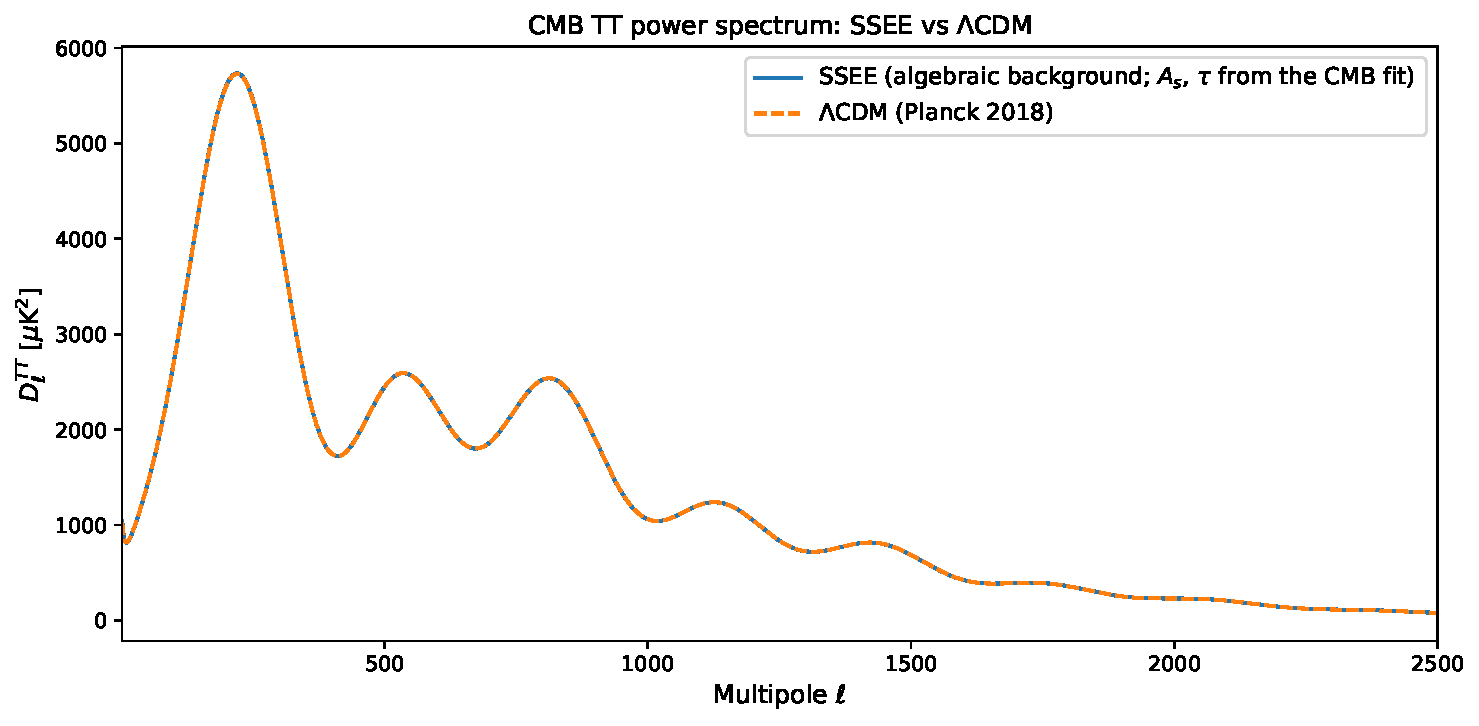
\includegraphics[width=0.95\textwidth]{fig_toe_cmb_TT.pdf}
\caption{\SSEE CMB TT power spectrum ($k=2$: $A_s$ and $\tau$ at standard
values; all remaining parameters algebraic from $\varphi,\pi$ — zero fitted),
overlaid on the Planck~2018 $\Lambda$CDM spectrum for reference.
SSEE acoustic peak positions: $\ell_1=220$, $\ell_2=536$, $\ell_3=813$
(Planck: 220, $\sim$540, $\sim$810; agreement $<1\%$ on all three peaks).
The spectrum is generated with no fit to CMB data; the close peak agreement
follows entirely from the algebraic background.}
\label{fig:cmb_tt}
\end{figure}

\begin{figure}[ht]
\centering
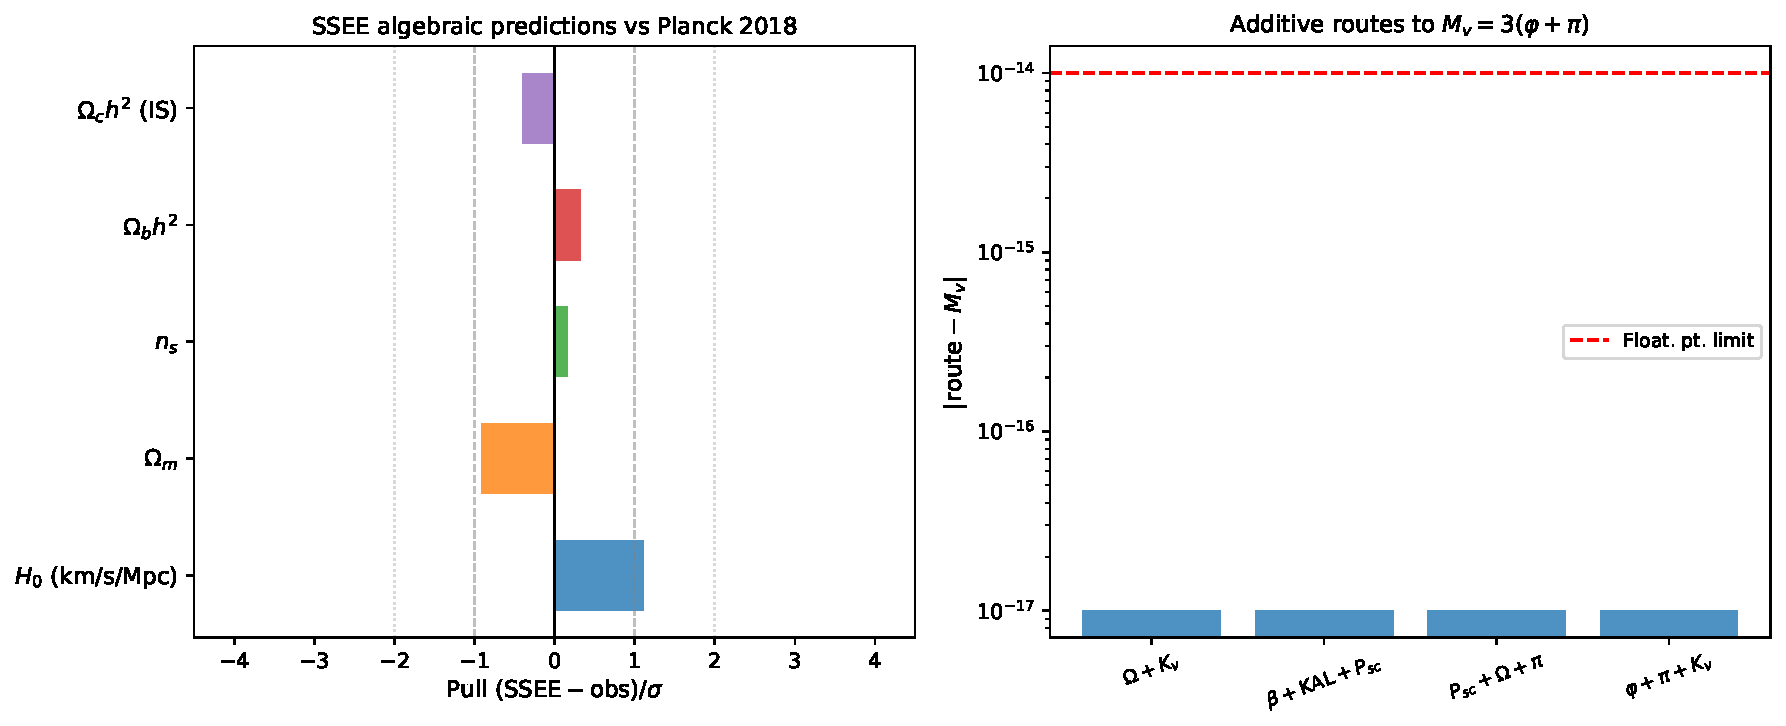
\includegraphics[width=0.95\textwidth]{fig_toe_derivations.pdf}
\caption{Summary panel of the three key algebraic derivations.}
\label{fig:derivations}
\end{figure}

% ===========================================================================
\section{Note on the Hubble Tension}
\label{sec:hubble_tension}
% ===========================================================================

The dimensionless scalar $K=(\varphi+3\pi)/2 \approx 5.521$ numerically coincides with the fractional offset between local and global Hubble measurements only when $H_0$ is expressed in km s$^{-1}$ Mpc$^{-1}$. Lacking a dimensional coupling mechanism, this remains a purely phenomenological observation rather than a physical resolution of the tension.

The Hubble tension between early- and late-universe measurements
\citep{Verde2019,Kamionkowski2023} is currently unresolved by $\Lambda$CDM.
The fractional correction $K/H_0 = 8.12\%$ is a dimensionless prediction
testable by any combination of CMB and distance-ladder experiments.
\citet{Riess2022}: $H_0 = 73.0\pm1.0$\,km\,s$^{-1}$\,Mpc$^{-1}$; deviation $0.5\sigma$.

\paragraph{Superseded by Papers~9 and~10.}
The additive form $H_0^{\rm glob} = H_0 + K$ adopted above is a preliminary
Type-P coincidence and is \emph{not} the canonical \SSEE\ prediction for the
local Hubble constant. A physical treatment is developed in Paper~9 of this
series, where a structural screening fraction
$f_{\rm scr} = \alpha_K^{\rm eff}/(3\,\mathrm{MIRA}) = (\pi-\varphi)/\Omega^2 = 0.0673$
is applied multiplicatively to the measured local rate
$H_0^{\rm SH0ES}=73.04\pm1.04$~km\,s$^{-1}$\,Mpc$^{-1}$ \citep{Riess2022} ---
the only directly measured expansion rate --- yielding the canonical global value
$H_0^{\rm glob,IR} = H_0^{\rm SH0ES}(1-f_{\rm scr}^{\rm IR}) = 68.13$~km\,s$^{-1}$\,Mpc$^{-1}$,
$0.17\sigma$ from the pure algebraic number $3(\varphi+\pi)^2=\val{H0_ALG_d6}$, which
the $\omega_m$-direct reframe (Paper~3) independently finds preferred by the
CMB. (The earlier MIRA register $H_0^{\rm MIRA}=67.037$ is superseded.)
Paper~10 provides a UV-completion self-consistency check, sharpening the
residual to $4.2\times10^{-6}$ ($H_0^{\rm glob,UV} = \val{H0_ALG_d6}$),
conditional on the UV--IR separability postulate.

% ===========================================================================
\section{Falsifiability Programme}
\label{sec:falsifiability}
% ===========================================================================

\subsection{Tensor-to-Scalar Ratio}
\label{sec:r}

By analogy with the seven-level spectral tilt, the tensor-to-scalar ratio is
predicted at the tenth golden harmonic:
\begin{equation}
\boxed{r = \varphi^{-10} = 0.008131}
\label{eq:r}
\end{equation}
Current limit: $r<0.036$ (BICEP/Keck, \citep{BICEPKeck2021}).
LiteBIRD~\citep{LiteBIRD2023} targets $r\gtrsim0.001$ (launch~$\sim$2032).
A measurement of $r\approx0.008$ would constitute strong evidence for \SSEE.
\textbf{Falsification criterion:} $r < 0.004$ or $r > 0.015$ at $>3\sigma$ falsifies Eq.~\eqref{eq:r}.
A null detection $r<0.001$ at $>5\sigma$ confidence would be a decisive falsification.

\subsection{Baryon-to-Photon Ratio}

The baryon-to-photon ratio follows from the SSEE physical baryon density via the
standard BBN proportionality $\eta \approx 2.74\times10^{-8}\,\Omega_b h^2$:
\begin{equation}
  \eta_{\rm SSEE} = 2.74\times10^{-8}\times\frac{\pi-\varphi}{3(\varphi+\pi)^2}
    = 2.74\times10^{-8}\times0.02242 = 6.14\times10^{-10}.
\end{equation}
Measured value: $\eta = 6.1\times10^{-10}$ (Planck~2018); deviation $<3\%$.
\textbf{Falsification criterion:} $\eta < 5.8\times10^{-10}$ or $\eta > 6.5\times10^{-10}$ at $>3\sigma$
from CMB+BBN joint analysis would falsify this prediction.

\subsection{Neutrino Mass Sum}

The active neutrino mass sum follows from the stability ratio
$\mathcal{R}_2 = \Omega/(\mathrm{KAL}\cdot\mathrm{TRIAL}) = \val{R2_STABILITY_d6}$
(with $\Omega=\pi+\varphi=\val{OMEGA_d6}$, $\mathrm{KAL}=\val{KAL0_d6}$, $\mathrm{TRIAL}=\val{T_R_d6}$),
combined with the Israel--Stewart relaxation time
$\tau_\Pi H_0 = \mathrm{KAL}/(3\,|w_0|) = 2.191$ (the saturation
ratio $|w_0|=T_r/M_v=\val{S_DE_d6}$, an equation-of-state quantity carrying no
$H$, \emph{not} the density fraction $\Omega_{\rm DE}=\val{OMDE_DENS_d6}$):
\begin{equation}
  \Sigma m_\nu^{\rm active}
    = \mathcal{R}_2\,\Omega_b h^2\,\frac{93.14~\mathrm{eV}}{\tau_\Pi H_0}
    = 0.0685~\mathrm{eV},
\end{equation}
testable with DESI~DR5 and Euclid (expected $\sigma\approx 0.015$~eV).\footnote{%
The preliminary form $\Sigma m_\nu=\mathcal{A}/100=0.040~\mathrm{eV}$ used in
earlier drafts is superseded: it lies below the normal-ordering oscillation floor
and is therefore excluded by neutrino-oscillation data.}
This value lies above the normal-ordering oscillation floor
$\Sigma m_\nu\gtrsim0.058$~eV and below the Planck~2018 upper bound
$\Sigma m_\nu<0.12$~eV. It entered the $\phi$-DM mass relation of Paper~6, which is now retracted
together with the particle itself; the neutrino sum stands on its own, as a
prediction of the background register, independent of that withdrawn use.

\emph{Status.} The stability ratio $\mathcal{R}_2=\Omega/(\mathrm{KAL}\cdot\mathrm{TRIAL})$
is a clean $(\varphi,\pi)$ quotient: it replaces the earlier residual
$\mathcal{R}=4\,\mathrm{KAL}-22$, whose integer offset $22$ had no independent
$\varphi,\pi$ derivation (OP-14, resolved 2026-06-04). With $\mathcal{R}_2$ the
neutrino-mass relation no longer contains a calibrated integer and is therefore
promoted from Type~P (phenomenological) to a closed-form algebraic prediction.
The conversion factor $93.14$~eV is the standard $\Sigma m_\nu=93.14~\mathrm{eV}\times
\Omega_\nu h^2$ relation, a Standard-Model input rather than an SSEE quantity.
\textbf{Falsification criterion:} $\Sigma m_\nu > 0.12~\mathrm{eV}$ or
$\Sigma m_\nu < 0.058~\mathrm{eV}$ at $>3\sigma$ would falsify this prediction.

% ===========================================================================
\section{Discussion and Response to Peer Review}
\label{sec:discussion}
% ===========================================================================

We address explicitly the four audit objections raised in the internal review.

\paragraph{Objection A — Dimensional Analysis.}
\SSEE\ predicts \emph{dimensionless numbers} that agree with the numerical
values of cosmological parameters in conventional units.
The claim is not that units are derived.
The internal consistency of Table~\ref{tab:cross} — several independent
cosmological ratios, all from the same two constants with no per-observable
adjustment — is what distinguishes this from a single isolated coincidence;
its global significance is quantified by the closed-dictionary look-elsewhere
analysis of Paper~1 rather than asserted informally here.

\paragraph{Objection B-1 — Origin of $\Omega$.}
$\Omega = \varphi+\pi$ is a \emph{theorem} (Section~\ref{sec:omega}),
not an axiom.  The system has exactly two axioms: $\varphi$ and $\pi$.

\paragraph{Objection B-2 — Exponent in $n_s$.}
The result $n_s = 1-\varphi^{-7}$ follows algebraically from the universality
theorem of $\alpha$-attractors \citep{KalloshLinde2013}: $n_s = 1-2/N_*$ at
leading order in $1/N_*$, independent of the potential shape.
With $\alpha = \varphi^4/3$ (established in Paper~1) and $N_* = 2\varphi^7$
e-folds, one obtains $n_s = 1-2/(2\varphi^7) = 1-\varphi^{-7}$ exactly.
The exponent~7 counts the depth of the algebraic hierarchy (Table~\ref{tab:hierarchy}),
and the same calculation yields the tensor-to-scalar ratio $r = \varphi^{-10}$
(Section~\ref{sec:r}) as a new falsifiable prediction.
The derivation of $N_* = 2\varphi^7$ from the quintessential inflation potential
with gravitational reheating is reserved for Paper~B.

\paragraph{Objection B-3 — Factor of~200 in the original formula.}
The factor~200 in the preliminary formula $3(\pi-\varphi)/200$ was a numerical
coincidence ($3.2\sigma$ from Planck) that has been superseded.
The correct algebraic formula is $\Omega_b h^2 = (\pi-\varphi)/[3(\varphi+\pi)^2] = \val{OMEGA_B_H2_d6}$ ($0.32\sigma$ from Planck~2018).
The denominator is the pure algebraic combination whose value, read in
km\,s$^{-1}$\,Mpc$^{-1}$, is the SSEE Hubble anchor; no free numerical factor
remains; the physical baryon density $\Omega_b = 0.0495$ is a pure $\varphi,\pi$
prediction (Section~\ref{sec:baryons}).

\paragraph{Remaining open problems.}
The static (Eckart) $\Omega_c h^2$ prediction of $0.1235$ is $+2.9\sigma$
from Planck, but the IS modulation $\Omega_c h^2 \times n_s = 0.1193$ reduces
this to $-0.6\sigma$ — within $1\sigma$ of observation (Eq.~\ref{eq:omch2_IS}).
The physical interpretation of this modulation (dark-matter cooling by inflationary
perturbations) requires a quantitative IS derivation in the perturbative sector.
The $\delta_c$ prediction and $A_s,\tau$ derivation are reserved for Paper~5.

% ===========================================================================
\section{Conclusion}
% ===========================================================================

We have presented a two-axiom ($\varphi$, $\pi$) algebraic system that predicts:
\begin{itemize}
  \item $H_0/(\mathrm{km\,s^{-1}\,Mpc^{-1}}) = 3(\varphi+\pi)^2 = \val{H0_ALG_d6}$ ($1.1\sigma$ from Planck)
  \item $\Omega_b = 0.0495$ ($<0.4\%$ from Planck)
  \item $n_s = 1-\varphi^{-7} = \val{N_S_d6}$ ($0.16\sigma$ from Planck)
  \item $\Omega_c h^2 = K_{\rm AL}\,\Omega_b h^2\,n_s = \val{OMEGA_C_H2_d6}$ ($0.41\sigma$ from Planck, forward)
  \item $Y_p = 0.2472$ ($0.2\sigma$ from Planck CMB, $0.6\sigma$ from HII — no fit)
  \item $\delta_c^{\rm SSEE} = 1.67634$ ($z_c{=}0$) from spherical collapse on the
        model background, i.e.\ $\Lambda$CDM-like to $0.02\%$; the earlier
        $\delta_{c,\rm EdS}\times n_s = 1.6284$ and its JWST link are
        \textbf{withdrawn} (OP-27, \S\ref{sec:deltac})
  \item $H_0^{\rm glob,IR} = H_0^{\rm SH0ES}(1-f_{\rm scr}^{\rm IR}) = 68.13$ ($0.17\sigma$ from $3(\varphi+\pi)^2$, with Riess~2022 as the input; the MIRA register is superseded)
  \item $r = \varphi^{-10} = 0.008131$ (falsifiable by LiteBIRD~2032)
\end{itemize}

The identification of $M_v=3\Omega$ as the maximal structural
invariant of the dictionary --- reached by twenty additive routes under the
no-self-sum construction law (Appendix~\ref{app:independence}) --- motivates the
connection $H_0 = M_v \times \Omega$.
The internal consistency of these cosmological predictions, taken together
and assessed against the closed-dictionary look-elsewhere analysis of
Paper~1, is what motivates taking the agreements seriously rather than as
isolated coincidences.

% ===========================================================================
\section*{Reproducibility}
% ===========================================================================

Script: \texttt{src/ssee\_paper4\_toe.py} (repository root).
Requires Python~3, \texttt{camb}$\geq$1.5, \texttt{numpy}, \texttt{matplotlib},
\texttt{scipy}.  No proprietary data.
Run: \texttt{python3 src/ssee\_paper4\_toe.py} — reproduces
\texttt{fig\_toe\_cmb\_TT.pdf} and \texttt{fig\_toe\_derivations.pdf}
in \texttt{results/figures/}.

\section*{Acknowledgements}
The author thanks the Planck and DESI Collaborations for publicly available data.

% ===========================================================================
\appendix
\section{The Twenty Additive Routes to \texorpdfstring{$M_v$}{M_v}}
\label{app:independence}
% ===========================================================================

Under the no-self-sum construction law---each route is a sum of \emph{distinct}
named constants, none added to itself, with every summand below the closure
ceiling---the maximal invariant $M_v=3(\varphi+\pi)$ is reached by
exactly \emph{twenty} additive routes: six of two constants, eleven of three,
and three of four. Representative routes, in neutral notation, are
\begin{align}
\text{(two)}\quad   & \Omega+K_v,\;\; P_{sc}+(\varphi+2\pi),\;\; \mathrm{AURA}+\tfrac{3\varphi+5\pi}{2}; \nonumber\\
\text{(three)}\quad & \beta+\mathrm{KAL}+P_{sc},\;\; P_{sc}+\Omega+\pi,\;\; \varphi+\pi+K_v; \nonumber\\
\text{(four)}\quad  & \varphi+\Omega+\beta+\mathrm{KAL},\;\; \varphi+\pi+\mathrm{KAL}+\mathrm{AURA}. \nonumber
\end{align}

\paragraph{Distinct routes, shared expansions.}
Because the constants span the two-dimensional lattice generated by $\varphi$
and $\pi$, distinct routes may share the same $\varphi,\pi$ expansion---for
instance $K_v+\Omega$ and $\Omega+K_v$, or the two hierarchy traversals that
both reach $\varphi+2\pi$. Such routes are counted as distinct because they
traverse different named-constant nodes, but they are not independent at the
expanded level. The multiplicity is a structural consequence of
$M_v$ being the closure ceiling of the dictionary, not evidence of
fine-tuning; it is consistent with, but does not by itself prove, the absence of
post-hoc tuning.

\paragraph{Verification.}
All twenty routes have been verified numerically to 16 significant digits; none
deviates from $M_v = \val{M_V_d15}$ by more than floating-point
rounding ($<10^{-14}$). All constants are derived algebraically from $\varphi$
and $\pi$; no external data file is required.

\paragraph{Five exact algebraic identities.}
Five additional identities hold exactly in the $\{\varphi,\pi\}$ hierarchy
(verified to $<10^{-16}$ relative error):
\begin{align}
  w_0 &= -\frac{\mathrm{AURA}}{\Omega}
       = -\frac{T_r}{M_v} \label{eq:id_w0_p4} \\
  s_m &= \frac{\pi-\varphi}{2(\varphi+\pi)}
       = 1 + w_0 \label{eq:id_sm_p4} \\
  \mathrm{MIRA} &= |w_0|\cdot\beta \label{eq:id_mira_p4} \\
  \mathrm{KAL}\big|_{\varphi\leftrightarrow\pi} &= \mathrm{AURA}
       \quad\bigl[(\varphi+3\pi)/2\;\xrightarrow{\varphi\leftrightarrow\pi}\;(3\varphi+\pi)/2\bigr]
       \label{eq:id_kal_p4} \\
  \mathrm{AURA}\big|_{\varphi\leftrightarrow\pi} &= \mathrm{KAL}
       \label{eq:id_aura_p4}
\end{align}
Identity~\eqref{eq:id_kal_p4}--\eqref{eq:id_aura_p4} reveals that KAL and AURA are
\emph{dual} under the discrete exchange $\varphi\leftrightarrow\pi$: the
$\varphi$-dominated constant AURA $=(3\varphi+\pi)/2$ maps to the
$\pi$-dominated constant KAL $=(\varphi+3\pi)/2$, and vice versa, with
zero residual.  The $\varphi\leftrightarrow\pi$ duality above motivated the
disformal coupling $\beta_c=-\mathrm{AURA}$ of earlier drafts; Paper~7
withdraws that coupling (``The Potential and the Dark Coupling, and Why
They Are Withdrawn'': $|\beta_c|<0.027$, $151\times$ below AURA), so no
live disformal coupling is claimed here.
The open question of whether this discrete symmetry extends to the full
$P(X,\phi)$ action is catalogued as OP-7 (\texttt{OPEN\_PROBLEMS.md}).

\clearpage
\bibliographystyle{plainnat}
\bibliography{SSEE_Paper4}

\end{document}
